%General formatting
\documentclass[oneside]{book}
\usepackage{amssymb,latexsym,color,amsthm}
\usepackage[margin=1.5in]{geometry}

%allows for comment blocks and verbatim sections
\usepackage{verbatim}
%For links
\usepackage{hyperref}
%For inserting images
\usepackage{graphicx}
%preserves tabs in verbatim sections. Good for including source code in documents.
\usepackage{moreverb}
%Clean version history
\usepackage{vhistory}
%Getting rid of all obnoxious image floating
\usepackage{float}
%Getting rid of all obnoxious auto-indentation
\usepackage{parskip}

%For examples
\definecolor{Dark}{gray}{.20}
\definecolor{Light}{gray}{.80}
\newcommand{\commandline}[1]{\begin{center} \colorbox{Dark}{\textcolor{white}{#1}} \end{center}}
\newcommand{\exampleout}[1]{\begin{center} \colorbox{Light}{\textcolor{black}{#1}} \end{center}}

%For exercises                          (Could be made prettier)
\newtheorem{ex}{Exercise}[chapter]

% code block formatting
\usepackage{listings,color}
\definecolor{verbgray}{gray}{0.9}
\definecolor{shadecolor}{rgb}{.9, .9, .9}
\lstnewenvironment{code}{
    \lstset{backgroundcolor=\color{verbgray}, 
    frame=single,
    framerule=0pt,
    basicstyle=\ttfamily,
    columns=fullflexible}}{}


\begin{document}
%Title Page
\title{An Abridged Introduction to the UNIX Command Line}
\author{CSCI Student Mentors \--- Western Washington University}
\date{}

\maketitle
\tableofcontents
\newpage


% Start of the revision history table
\begin{versionhistory}
    \begin{center}
        \large{\textbf{Version 1.0 from 4/24/16}}
    \end{center}
    \large{\textbf{Authors:} Brandon Tarquinio(BT), Robin Cosbey(RC)  Ted Weber (TW), Sarah Gunderson (SG), Serena Bowen (SB)}
  \vhEntry{1.0}{4/24/16}{TW}{created}
  \vhEntry{1.1}{4/27/16}{TW, SG, SB}{revisions}
\end{versionhistory}
                                                    %Workshop 1
\chapter{The Basics}
\begin{center}
\framebox{Download this PDF at \url{www.com}}
\end{center}

\section{Introduction}
In this workshop we will run through the basics of using $bash$ or some other Unix-like command line environment. $bash$ is the most popular of the different $shells$ (it is then default on most Linux distros and OSX) but most things we discuss will be universal to all shells for Unix-like computers.\footnote{For example Linux, OSX, FreeBSD. Also Cygwin provides a Unix-like environment for Windows computers.} 

\section{What is a shell?}
In general, a shell is a user interface for accessing the operating system's services. This includes command line interfaces (like \textit{bash}), as well as graphical shells that provide graphical user interface built on top of a windowing system.\footnote{More information about shells here \url{https://en.wikipedia.org/wiki/Shell_(computing)} and the history of shells here \url{https://www.ibm.com/developerworks/library/l-linux-shells/}} 

\begin{figure}[H]
	\centering
	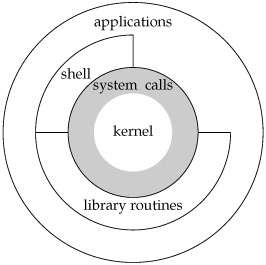
\includegraphics[scale=0.5]{kernel.png}
	\caption{The shell sits above the kernel, which is generally the lowest-level, or "inner-most" component of most operating systems.} 
\end{figure}

\section{Getting started}
We will be focusing on using the command line interface, \textit{bash} is particular. This will include how to manipulate files and directories, use the built-in manual pages, compile/execute programs, and build your command repertoire in general. Let's start by opening the terminal:\footnote{Most Linux desktop environments use this keyboard shortcut by default, but it does vary. If this shortcut doesn't work you can use the search functionality in your desktop environment.}

\commandline{ctrl + alt + t}


%% Shorten this section

\section{Running a Command}
The general form of any command, for the most part, is as follows:
\commandline{\$ commandname -arg1 ... \ \\-\\-longerargs ... input1 input2 ...}
\begin{itemize}
    \item \textbf{\$} is what's known as your command \textit{prompt}, and it is display on the console after every command has finished executing.
    \item \textbf{commandname} refers to the name of the user command.
    \item \textbf{-arg} is an example of a \textit{short-option}, which is a single dash followed by a single character.
    \item \textbf{\texttt{-{}-}longerargs} is an example of a multi-character \textit{long-option}, and these are preceded by two dashed. \textit{These additional long and short-options are just extra features for the given user command.}
    \item \textbf{input1} and \textbf{input2} represent additional arguments, or parameters, that the user command may allow.
    \item The ``\dots" above are used to denote the fact that we can have multiple arguments and parameters for a single command.\footnote{In actuality every command has a finite number of arguments it understands and you normally use a small subset of those. There might also be a limit on the number of inputs.}
\end{itemize}
   
Lets look at an example:
\commandline{echo hello world}

\textbf{echo} is a simple command that displays a line of text. Now let's try adding an optional short argument.

\commandline{echo -n hello world}

the \textbf{-n} was interpreted by the shell as a \textit{short-option} telling the shell to refrain from putting a newline character ($\backslash$n) at the end of the input string.

\section{Directories and Moving Around}

\subsection{Directory trees and pwd}
We will start by learning some commands to move around the directory tree. It is called a directory tree because it can be visualized as follows:

\begin{figure}[H]
	\centering
	\label{tab:directory_tree}
	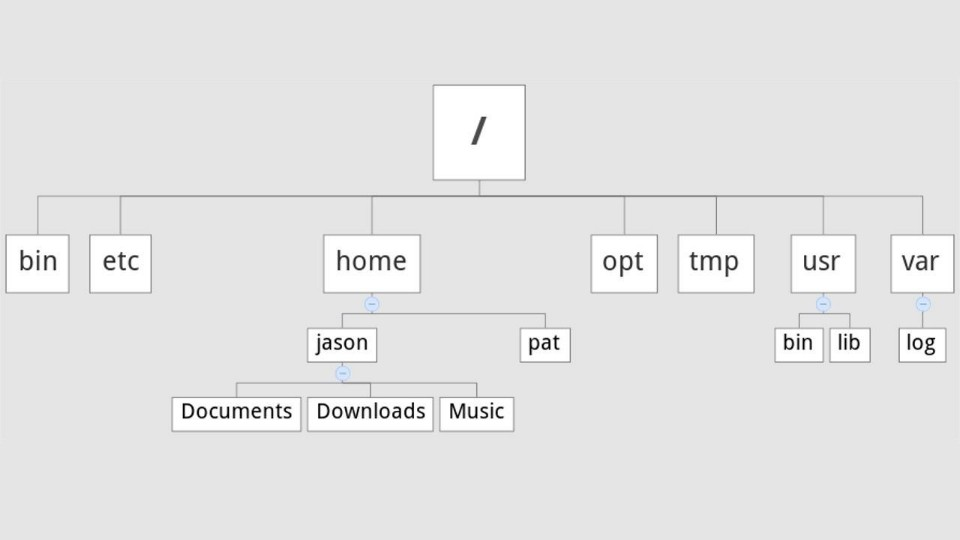
\includegraphics[width=90mm]{linux-directory-tree.jpg}
	\caption{An Example Linux Directory Tree.} 
\end{figure}

Each of the boxes in Figure 1 are directories and we call the directory ``$/$" $root$ since it is the root of our tree. In a command line enter:
	\commandline{pwd}
  This will \textbf{p}rint your current \textbf{w}orking \textbf{d}irectory. For example if we were in the home directory of the user $jason$ and typed \textbf{pwd} we would get the following:
	\exampleout {/home/jason}
	
A user's \textit{home directory} is the default current working directory when you open up a terminal. You can think of it as the root of your personal directory tree, different than the root of the entire file system.


\begin{ex} 
	Lets explore the concept of home by running the following commands:
	\commandline{pwd}
	\commandline{echo $\sim$ }
	What did you find? Note that ``$\sim$", the tilde symbol which is located to the left of the 1 on your keyboard. Remember ``$\sim$" since it will be used a lot as a shortcut to your home directory.
\end{ex}

\subsection{Listing the contents of a Directory}
To \textbf{l}i\textbf{s}t all the files in your current working directory enter:
	\commandline{ls}
	Most shell environments can be set up (and yours might already be) so that directories are printed with a different colour than files and directories shortly. We can also specify to \textbf{ls} what directory we want to list the contents of with the following generic form:
  	\commandline{ls dirname}
For example:
	\commandline{ls $\sim$}
will display the contents in your home directory.

To display more information about the files, use the \textbf{-l flag}:

\commandline{ls -l}

Example output:
\exampleout{-rw-r--r-- 1 webert3 grp.csci.Students 0 Apr 27 12:26 file1}
\exampleout{drwxr-xr-x 4 webert3 grp.csci.Students 4 Apr 25 14:11 java\_programs}

There is a lot more information here! So what does it all mean? Lets use the file listing for the directory \textit{java\_programs} as an example:

% ls -l information
\begin{center}
    \begin{tabular}{|c|c|c|c|c|c|c|c|}
        \hline
	    1 & 2 & 3 & 4 & 5 & 6 & 7 & 8 \\
	    \hline
        d & rwxr-xr-x & 4 & webert3 & grp.csci.Students & 4 & Apr 25 14:11 & java\_programs\\
        \hline
    \end{tabular}
\end{center}
	
\begin{enumerate}
    \item File type. For example, \textbf{-} for a file, \textbf{d} for a directory, or \textbf{l} for a link.
    \item File permissions. 
    \item Number of hardlinks to this file.
    \item Owner of the file.
    \item Group that the file belongs to.
    \item The size of the file in bytes.
    \item The date in which the file was last modified.
    \item The name of the file.
\end{enumerate}

We won't go into detail on the specific meaning of these fields in this workshop, but there is a link in the footnotes for more information.\footnote{Advanced Bash workshop: ADD LINK TO BASH II WORKSHOP ON GITHUB HERE!!!}
	
\subsection{Changing your Current Working Directory}
We have talked a lot about current directories changing but have yet to figure out how to do so. We can \textbf{c}hange the \textbf{d}irectory with \textbf{cd} which has the following form:

\commandline{cd dirToChangeTo}
For example we can run:
\commandline{cd /}
And then:
\commandline{pwd}
and we will see:
\exampleout{/}
To change back to our previous working directory with this shortcut:
\commandline{cd -}
To change to our home directory regardless of where we are we can simply type:
\commandline{cd}
Thus the default to \textbf{cd} is to change to the users home directory. \\
Lastly, to move back one directory in the directory tree enter this command:
\commandline{cd ../}

\begin{ex}
	Use \textbf{cd}, \textbf{pwd}, \textbf{ls} to explore the directory tree a bit. Becoming familiar and quick with this is key to become efficient with the command line since \textbf{cd} and \textbf{ls} are easily the two most used commands.
\end{ex}

\subsection{Relative vs Absolute Path Names}
We need to learn one more important concept about UNIX files and directories before moving on to learning a bunch of commands and how we can use them to help us program. \\
Suppose we are in the directory /home in our directory tree figure and we wanted to list the contents of the jason directory. We can do this in two ways:
\commandline{ls jason}
or
\commandline{ls /home/jason}
In the later we used the \textbf{absolute path name} which is the name of the file or directory prefixed by the path from ``/" to it. When we use absolute path names it no longer matters what are current working directory is e.g. we could have run the second command from any directory. In contrast, the first command will only list the contents of /home/jason if are current working directory is /home. This is because jason is a \textbf{relative path name} since we assume the path begins in our current working directory. Relative path names allows the user to remember and type less but require careful consideration of what your working directory currently is. 

\subsection{Special Directory Entries and Hidden Files}

Hidden files and directories are generally configuration files that are not shown unless you specify that you would like to see them. These entries are hidden to de-clutter the file system. Now we will review two important hidden directories that are useful shortcuts.

\begin{itemize}
	\item ``.": This represents the current directory and is an actual entry in every directory.
	\item ``..": This represents the parent of the current directory and is also an actual entry in the current directory.
\end{itemize}

\begin{ex}
	Navigate to the directory \textit{dirs} in the demo files you downloaded from GitHub. Now enter the following commands 
	\commandline{ls -a}
	\commandline{ls -a .}
To view all files in your home directory:
	\commandline{ls -a $\sim$}

Does the output make sense? As a challenge question what will the following command do? (Try to think it out before running it!):
	\commandline{ls ././././}
\end{ex}

\section{Grab the Demo Files from GitHub!}
Take a moment to download a few files for this workshop from our GitHub. Each lab machine has the version control system Git installed, so if you enter the following command you will download our demo files into your current working directory.

\commandline{git clone [put the link here...]}
\commandline{cd demo}

\subsection{Making a Directory}
Now that we understand the directory tree and how to move around it we are ready to learn how to add to it. The general form of the command to \textbf{m}a\textbf{k}e a \textbf{dir}ectory is:
\commandline{mkdir newdirname1 newdirname2 ...}
\begin{ex}
	Run the following sequence, before the second and third call to \textbf{ls} think about what you would expect to see:
\commandline{clear}
\commandline{ls}
\commandline{mkdir FirstDir SecondDir}
\commandline{ls}
\commandline{mkdir FirstDir/Foo FirstDir/Foo2}
\commandline{ls FirstDir}
\textbf{clear} is a useful command that clears the screen.
\end{ex}

\subsection{Creating a File}

Unix is very flexible regarding file names. A valid Unix file name can contain any other character than ``$\backslash$". Also, Unix does not add any special significance to characters like ``." or ``$\_$" in file names; they are treated like any other character. You can create an empty file using the command \textbf{touch}.
\commandline{touch file_name}

\begin{ex} In this exercise you will create an empty hidden file.
    \begin{enumerate}
        \item Create a file called \textbf{.f1}.
        \item Try finding the file using \textbf{ls}.
    \end{enumerate}        
\end{ex}


\subsection{Deleting Files \& Directories}
The program to \textbf{r}e\textbf{m}ove a file or directory is \textbf{rm}, and it has the following form:
\commandline{rm [OPTION] ... [FILE]...}

\textbf{IMPORTANT NOTE:} With great power comes great responsibility. This command will remove a file from your file system permanently. THIS COMMAND DOES NOT PUT FILES INTO A TRASH/RECYCLING BIN. There may be some way to recover files after using \textbf{rm}, but it will not be easy, especially for an inexperienced user.\footnote{\url{https://unix.stackexchange.com/questions/101237/how-to-recover-files-i-deleted-now-by-running-rm}} Be cautious! \\

Also, by default this command only works if the directories you are trying to delete are \textbf{empty}. An empty directory is a directory which only has no other entries but ``." and ``..".

If you would like to delete a directory and all of it's contents, use the \textbf{-r} flag.\\
\commandline{rm -r FirstDir} 

This will silently remove FirstDir/Foo, FirstDir/myfile, and FirstDir/Foo2 forever. \textbf{AGAIN}, this is a powerful tool, don't blow away your entire file system but running this command on your home directory!\footnote{The WWU CS Mentors are not liable for any misuse of this command. Sorry folks!} 

If you want to play it safe, use the \textbf{-i} flag and a prompt will come up before removal.\ 
\commandline{rm -i file1}

\section{Basic Shortcuts}

\subsection{clear}
Is your terminal covered in lines of code and difficult to determine where one previous command ends and another begins? Typing ``clear" into the terminal will wipe away all of the old commands (command shown below).
\commandline{clear}
It is possible to refer back to those deleted commands by scrolling up in the terminal.

\subsection{ctrl ($\wedge$)}
Sometimes within bash ctrl will be denoted by `` $\wedge$ ". Ctrl is included with several commands, one of the more relatable being ctrl-C. This will terminate the process. 

\subsection{tab completion}
When we enter tab at the prompt it will try to finish whatever we are currently typing as long as there are no ambiguity. For example if we only had ``\textbf{file1}" in our current working directory we could view the file listing by tying ``\textbf{ls f}" and hitting tab. It will fill out the rest of the word so that you now see:
\commandline{ls file1}
If instead we had both ``file1" and ``file2" then when we pressed tab it would have only filled in this much:
\commandline{ls file}
This is because it does not know if you want a 1 or a 2 to follow next. To see all option press tab twice and the list of all options will be displayed on the screen.\\

\begin{ex}
    Tab completion can also be used to complete program names as well.
    \begin{itemize} 
        \item Type \commandline{py}
        \item Use tab completion to complete the command ``python" and launch an interactive python shell.
        \item Exit the python shell by typing \commandline{exit()}
    \end{itemize}
\end{ex}

\subsection{Wildcard expansion (*)}
The \textbf{*} symbol is known as a wildcard. This is a useful tool in various situations, but is commonly used to perform actions on more than one file at a time, or to find part of a phrase in a text file.\footnote{Standard wildcards are also known as globbing patterns. For more information see \textbf{man 7 glob}.} 

Lets give it a try by navigating to the directory \textit{demo/dirs} and typing this command:
\commandline{ls -l f*}

You should see the extended file listings for all three files!

\section{Editing Files}
 In Computer Science courses we will use files for lots of reasons:
\begin{itemize}
	\item Your Program source code: Whether you are taking a class in Python, Java, C, or some other language you will need a file that is your program.
	\item Programs themselves: In Unix, all of the programs, the ones you write and the ones that are installed, are themselves a file. For example type the following commands:
		\commandline{which ls}
		\commandline{which python}
		\commandline{which which}
	\textbf{which} is a command that tells you where the program is in the computer. It is especially useful in the case of python since most computers have multiple versions of python and which can tell you which python you use when you type python.
	\item Plain text files: For example, input to or output from your program will be saved in text files. 
\end{itemize}

% \subsection{Nano}
% \textbf{nano} is a basic command line editor that will come on almost any Unix computer you ever use. It is not the best for writing programs in but it is simple to learn. The following is generic way to make a new file with nano:
% \commandline{nano newfilename}
% It will open the editor full screen in your terminal. On the bottom you will see some of the commands you can use where the carrot (this symbol `` \^{}  ") represents the control key. You can enter text by just typing.
% \begin{ex} 
% 	In this exercise we will make a file with nano. \\
% 	\begin{enumerate} 
% 		\item If you are not already in FirstDir then change your directory to FirstDir. Remember you can check where you are with \textbf{pwd} and you can use \textbf{cd} to get to FirstDir.
% 		\item Now make a file named myfile using the following command:
% 			\commandline{nano myfile}
% 		\item Type the following line:
% 			\exampleout{I am making my first file in nano!}
% 		\item Saving: Notice on the bottom of the screen it says ``WriteOut" with a ``\^{}O" next to it? That is how we will save our file. Save by first hitting Ctrl+o and see that it prompts you for the file name on the bottom of the screen. Now hit enter. We should now see a new message on the bottom of the screen saying ``Wrote 1 line".
% 		\item Exiting: Now that we have saved some text lets leave by hitting Cntr+x. Now we are back on the command line.
% 		\item Use \textbf{ls} to check if our file is in FirstDir. 
% 		\item Check the contents by using the \textbf{cat} command as follows ( we will learn more about reading text files in the next section):
% 			\commandline{cat myfile}
% 		\item Edit the file to have the following line added on the next line of the file
% 			\exampleout{I am editing my file to have 2 lines}
% 			by entering
% 			\commandline{nano myfile}
% 		\item Now add a third line of whatever you like.
% 		\item Now save and exit. Also use \textbf{cat} again to see your changes.
% 	\end{enumerate}
% \end{ex}
% That is about all you need to know to make some simple files using nano.

% \subsection{Vim}
% Another editor that will always be present in a Unix environment is the program \textbf{vi} or it's big brother \textbf{vim} which stands for \textbf{v}i \textbf{im}proved. \textbf{vi} and \textbf{vim} are much more powerful than nano but have a much steeper learning curve. In turn we will have a dedicated workshop on how to use them. For now we will give the bare minimum. You can edit a file called ``myvimfile", or make one if that file does not already exist, with the following command:
% \commandline{vim myvimfile}
% This will open up a full screen editor similar to what happened with nano. You will notice tilde characters along the left side which signify that those lines are not part of your text file. There is also a bar along the bottom that will tell you the name of your file along with it's length (or in the case of a new file it will say ``[New File]"). We are currently in a Command Mode which means that what we type will not be entered on the text file but instead give commands to Vim. There are many things we can do in this mode but in this workshop we will only learn how to type. Hit the i key to enter \textbf{I}nsert Mode. You can now type exactly like you would in any other text editor. \\
% First hit i and notice the bottom line change to have the following on the left side:
% \exampleout{--  INSERT  --}
% This will be there whenever we are in Insert Mode. Enter some text such as the following:
% \commandline{ Here is a line of text that I entered in Vim}
% To leave Insert Mode hit the Esc key. Notice that the bottom has changed to be blank on the left, this means that we left Insert Mode. Now to save, or \textbf{w}rite, our changes and leave, or \textbf{q}uit, Vim enter the following:
% \commandline{:wq}
% After you hit enter you should be back at the command line with your new file in your current working directory.
% \begin{ex}
%     This assignment is too long to do during this workshop but when you get home enter the following to beginning a tutorial of how to use Vim:
%     \commandline{vimtutor}
%     This tutorial last about 20 minutes and gives you enough to be able to start editing files with Vim using some of vim's power. If you are interested in learning more you should also visit our Vim workshop later this quarter.  
% \end{ex}


\subsection{Others}
There are several pure command line editors like \textit{vim} and \textit{emacs}, but we will refrain from using these in our demo because there is some overhead to learn these tools. We can also use the command line to open up one of our favorite gui\footnote{gui stands for \textbf{G}raphical \textbf{U}ser \textbf{I}nterface} text editors with commands like: 
\commandline{gedit myfile}
\commandline{atom myfile}
Note that when you run one of the above commands it may open a gui window and you will no longer be able to use the command line until you close the newly opened window. You can get around this by doing the following:
\commandline{gedit myfile \&}
This will open gedit (or whatever program you choose) in the $background$ and allow you to continue using the command line. \\

\begin{ex} Create a file and write to it.
    \begin{enumerate}
        \item Open up a gui text editor, or command line editor if you have experience.
        \item Write some characters in the file.
        \item Save your changes (writing your data to the disk).
        \item Find out how large your file is in bytes (do you remeber what command to use?).
    \end{enumerate}
    
\end{ex}

\section{More on Files}

\subsection{Reading Files}
	There are many ways to read files; we will discuss a few now. For starters you can always use a program you use to editing text files with to read a file (for more on this see the Editing Files section). In general though you should use the right tool for the right job and if you don't want to edit a file you should use a viewer such as \textbf{less} or \textbf{more}.
	For example, to open the file $myfile$ with \textbf{less} type:
\commandline{less myfile}
This will open the file full screen in the command line and allow you to move up and down the document line by line. You can do this by pressing the up and down arrow keys. For those familar with Vim you can use Vim's way of moving around in less (which is why less is so cool!). Also some terminals are set up so you can use the scroll wheel on your mouse. 


To use \textbf{more} to open the file $myfile$ type:
\commandline{more myfile}
This program is more primitive and is mostly used for reading though large chunks at a time instead of normal viewing. Hit space to move to the next page until you are done or press q to \textbf{q}uit at any time.\footnote{Pressing q to quit is also used in less.} So yes,  \textbf{less} actually has more functionality than the command \textbf{more}.

Some other ways of viewing include \textbf{cat}, \textbf{head}, and \textbf{tail}. cat's main purpose is for con\textbf{cat}ination but it can also be used to dump a file to the screen by typing:
\commandline{cat myfile}
This is great for small files but horrible for larger ones. \textbf{head} and \textbf{tail} will grab the first or last 10 lines, respectively.\footnote{These commands has several other options as well allowing you to grab a variable number of lines. See \textbf{man 1 tail}}.\\

\begin{ex} Try running these commands on the file ``numbers"
\commandline{cat numbers}
\commandline{more numbers}
\commandline{less numbers}

\end{ex}

\subsection{Copying a File}
We can \textbf{c}o\textbf{p}y a file by \textbf{cp} command which has the following generic form:
\commandline{cp sourceFileName destinationFileName}
For example:
\commandline{cp myfile myfile.backup}
will make it so the file name $myfile$ in my current working directory is copied into a new file called $myfile.backup$ which will also be in my current directory.

\subsection{Moving a File}
We can \textbf{m}o\textbf{v}e a file by the \textbf{mv} command which has the following generic form:
\commandline{mv sourceFileName distinationFileName}

\begin{ex} Copy a file, then move the copy elsewhere.
    \begin{enumerate}
        \item Create a file using \textbf{touch}.
        \item Make a copy of the file using \textbf{cp}.
        \item Use \textbf{mv} to move the copied file to a new file within the same directory. That is, run a command of the following form:
        \commandline{mv file.copy file.newfile}
    \end{enumerate}
Tip: Run \textbf{ls} before and after the command and observe the result.
\end{ex}

\subsection{Rename?}
There is no rename command since the effect of such a command can already be achieved by something we already learned.
\vspace{0.3cm}

\begin{ex}
	Try renaming a file using one of the commands we've already learned. \textbf{SPOILER}: We renamed a file in the previous exercise!
\end{ex}	

% \subsection{Deleting a File}
% To \textbf{r}e\textbf{m}ove a file we can use \textbf{rm} which has the following form:
% \commandline{rm fileName fileName2 ...}
% Again be careful with this command since it will not prompt you about if you really want to delete and it will delete it for good. There is an even more powerful and dangerous version of rm when we supply the -r argument\footnote{r is for \textbf{r}ecursive} which given a directoryname as input will delete the directory and everything in it. 
% Thus (\textbf{DO NOT DO THE FOLLOWING COMMANDS}):
% \commandline{rm FirstDir}
% and
% \commandline{rmdir FirstDir}
% will result in errors but:
% \commandline{rm -r FirstDir} 
% will silently remove FirstDir/Foo, FirstDir/myfile, and FirstDir/Foo2 forever. This solves the problem we had earlier of how to delete a non-empty directory. 
% \begin{ex}
% 	\begin{enumerate}
% 		\item Change your current working directory to FirstDir/Foo.
% 		\item Now use nano to make a file named file1 with a couple lines and use vim to make file2 with a few lines.
% 		\item Delete file1 and file2. Can you do it with 1 command?
% 		\item Change your directory back to FirstDir and create a new directory in Foo called Bar.
% 		\item Add some blank files with the following command:
% 		    \commandline{touch Foo/afile Foo/anotherfile Foo/onemorefile}
% 		\item List the contents of Foo.
% 		\item Run the following exactly:
% 		    \commandline{rm -r Foo}
% 		\item What was the result?
% 	\end{enumerate}
% \end{ex}

\section{Manuals}
In this section we will learn how to learn new things about the command line without ever having to leave it! This includes how to learn more about commands we already know and how to find new commands.
\subsection{ A help message}
Many Unix programs will use one or both of the following to give you a brief help message:
\commandline{program\_name -h}
or
\commandline{program\_name \ \\-\\-help}
This is optional so some programs will have both, one, or neither of the above arguments. Also some programs that have both will have different messages for each. Note that some programs will also use -h to do something other then give a help message.
begin{ex}
Try them with \textbf{vim}:
	\commandline{vim -h}
	\commandline{vim \ \\-\\-help}
	Now try them with \textbf{ls} and \textbf{which}.

We have learned that -h and --help sometimes give brief help messages but we also found flaws with consistency. A more consistent system with verbose messages are the programs \textbf{man} and \textbf{info}.
\subsection{Man Pages}
The \textbf{man} program gives you \textbf{man}ual pages about what every program you specify. Its general form is:
\commandline{man program\_name}
For example:
\commandline{man cat}
will give you information on the program \textbf{cat} which we have seen a few times now. You can even learn more about \textbf{man} by running the following:
\commandline{man}
The interface for reading these pages is the same as \textbf{less} so this should feel familiar by now. For those who use C note that you the system calls and libc functions have manual pages in section 2 and 3 of the man pages! 
There are nine sections to the man pages and sometimes two things with the same name will exist in different sections. For example:
\commandline{man printf}
will open a manual page for a program called \textbf{printf} which is not an important command to learn but merely a good example. We can see that this is from the first section due to the top left corner having this:
\exampleout{PRINTF(1)}
The number in parenthesis is the section the page is in. Thus we get the same page if we instead type:
\commandline{man 1 printf}
Now those who have ever written a line of \textbf{C} will no that this is the name of a library function to print text to the screen. To view the page for that function enter the following:
\commandline{man 3 printf}
See how it is a different page? The manual is generally split into eight number sections:

\begin{center}
    \begin{tabular}{|c|c|}
        \hline
	    1 & User commands \\
	    \hline
        2 & System calls \\
        \hline
        3 & Library functions \\
        \hline
        4 & Special files \\
        \hline
        5 & File formats \& conventions \\
        \hline
        6 & Games and screensavers \\
        \hline
        7 & Miscellanea \\
        \hline
        8 & System administration commands and daemons \\
        \hline
    \end{tabular}
\end{center}

We have been mostly dealing with \textit{user commands}, but if you were writing a \textbf{C} program you would likely be visiting section 2 and section 3 quite frequently.\\

\begin{ex} Using the man pages.
    \begin{enumerate}
        \item Try opening the man page for a command we have previously used.
        \item Try using this command with one of the listed long or short-options. 
    \end{enumerate}
\end{ex}


\subsection{Info Pages}
\textbf{man} pages are the standard way of learning how use software on Unix systems and it cannot be stressed enough how important it is to learn how to use. As stated before \textbf{man} uses the \textbf{less} program to view the pages and thus it has a way of interacting that is similar to \textbf{vim}. There is a newer program and set of \textbf{info}rmational pages called \textbf{info} which instead uses the text editor \textbf{emacs} style of interacting. There are some programs that only have both \textbf{man} and \textbf{info} pages, only one, or neither. \\
View an info page by running:
\commandline{info program\_name}
You will get a full screen viewer like \textbf{man} but arrow keys and vim movements wont work! You can move forward pages with ``ctrl+v" and backward pages with ``alt+v" to view pages similar to \textbf{more}. You can move line by line by using ``ctrl+n" and ``ctrl+p" to move to the \textbf{n}ext and \textbf{p}revious lines respectively. You can leave by typing ``q" just like we did with \textbf{more}, \textbf{less}, and \textbf{man}. \\
\begin{ex}
	View the info page of some of the commands we have learned so far. Are there any differences? 
\end{ex}
Just like Vim, Emacs is a very powerful editor with a sharp learning curve that is loved by many programmers. We will offer workshops on both Emacs and Vim this year and encourage everyone to learn a bit about both editors. 

\subsection{Programs to help you find commands: \textbf{apropos} and \textbf{whatis}}
We can use the \textbf{whatis} program to get quick descriptions about other program. The general form is:
\commandline{whatis programname}
For example we can type:
\commandline{whatis ls}
and see:
\exampleout{ls (1)		- list directory contents}
The one should be familiar, it is the section of the man page that \textbf{ls} is in. If all of these descriptions are in the computer it would be cool to search for commands like you would use google to search for webpages.
That is what \textbf{apropos} is for, it has the following general form:
\commandline{apropos whatToSearchFor}
For example if we wanted to find other editors to use we could try:
\commandline{apropos editor}
This will produce a list of every command whose name either contains ``editor" or whose \textbf{whatis} description contains ``editor". Clearly this will not always contain the results you want and therefor you can try different searches to refine or expand your results such as:
\commandline{apropos text editor}
Also note that you can group words with quotation marks:
\commandline{apropos ``text editor"} 
Will only return results that have $text$ followed by $editor$ in the \textbf{whatis} description.

\subsection{When you just want to use your default}
The user command \textbf{xdg-open} will open a file or URL in the user's preferred application. For example:
\commandline{xdg-open `https://www.google.com'}

This will open \url{www.google.com} in your default web browser.

\section{Running Your Programs}
In this section we will show how to use the command line to run the programs we write. Since no assumptions are made as to how far you are in Western's Computer Science Department's curriculum we will show how to run programs in Python \& Java. All code will be provided so you can follow along without needing to know the language. For each one language we will run the iconic Hello World program.
\subsection{Python}
Change your current working directory to \textit{demo/python\_programs}, which should be already created for this demo.

Use a text editor to create and edit the following file called ``HelloWorld.py". For example:
\commandline{atom HelloWorld.py}

Write this in your file:

\commandline{print("Hello World!")}
 and save the file. Now on the command line enter the following to run your program:
\commandline{python HelloWorld.py}
This will open the python interpreter with the file ``HelloWorld.py" running on it. You should see the following output:
\exampleout{Hello World!}\\

\subsection{Java}
Change your current working directory to somewhere you would like to save your java programs. For our demo you could do this in the directory \textit{java\_programs}.

Create a file called ``HelloWorld.java" using your favorite text editor.:

\commandline{[some text editor] HelloWorld.java}

Write the following:

\begin{verbatimtab}
    public class HelloWorld {
        public static void main(String[] args) {
            System.out.println("Hello World!");
        }
    }
\end{verbatimtab}
and save the file. Now compile the program with the following:
\commandline{javac HelloWorld.java}
If errors occurred during compilation they would be displayed during the last step. You would need to fix the lines in the file causing the errors and rerun the previous line until your program compiles correctly. If the program compiles without errors you should see ``HelloWorld.class" when you enter:
\commandline{ls}
Now we can run the program with the following command:
\commandline{java HelloWorld}
Which, as you might expect, will display the following:
\exampleout{Hello World!}

\vspace{0.5cm}

\begin{ex}
    To see example of how errors will be displayed edit ``HelloWorld.java" to no longer have class on the first line. Recompile with the \textbf{javac} command we just learned. See how the top line that is returned informs us that java was expecting the world class but couldn't find it?
\end{ex}

% \subsection{C++}
% As before change to our C++ directory with:
% \commandline{cd ../C++}
% With an editor make a file called HelloWorld.cpp with the following content:
% \begin{verbatimtab}
%     #include <iostream>
%     using namespace std;
    
%     int main() {
%         cout << "Hello World!" << endl;
%     }
% \end{verbatimtab}
% C++ is a compiled language which means that we need to first compile it before we can run it. We can compile our new program with the following command:
% \commandline{g++ HelloWorld.cpp}
% Any errors will be displayed but if you copy my lines exactly you will see nothing except for a new prompt on the screen. List the contents of your current working directory to see a new file called ``a.out", this is the file which is our new program. We can run it with the following:
% \commandline{./a.out}
% The output should be exactly what you expect. 
% \begin{ex}
%     C++ defaults to compiling our program into a file called a.out but we can specify what we would like our program called with the following option to g++:
%     \commandline{g++ ourprogramfile.cpp -o whatIWantMyProgramToBeCalled}
%     Use this to compile ``HelloWorld.c" into a file called ``HelloWorld". How can we run this new program?
% \end{ex}

% \subsection{C}
% As before change to our C directory with:
% \commandline{cd ../C}
% With an editor make a file called ``HelloWorld.c" with the following contents:
% \begin{verbatimtab}
%     #include <stdio.h>
    
%     int main() {
%         printf("Hello World!\n");
%     }
% \end{verbatimtab}
% We can compile our C program with the compiler gcc using the following command:
% \commandline{gcc HelloWorld.c}
% This has very similar semantics to g++ including the same way it compiles to a file called a.out and how you can change this in the same way we learned in the C++ exercise. This is because they are essentially the same program. We again can run our new C program with the following:
% \commandline{./a.out}
% And that is the basics of how to run programs using the command line. There are many extra options to these commands but this minimum will allow you to make most programs.

\newpage
\section{More Shortcuts}
There are a number of shortcuts that save typing time and allow you to remember less. We will discuss a few now.
\subsection{Reuse previous commands}
You will notice the more you use the command line that there the same sequence of commands are used a lot. For example when you are writing a program you will edit it using nano, vim, or emacs and then compile or run the program. You will then notice a bug and open the editor again and then test your changes by compiling or running your program again. Such as:
\commandline{vim HelloWorld.c}
\commandline{gcc HelloWorld.c}
\commandline{./a.out}
\commandline{vim HelloWorld.c}
And this will cycle will keep going. Wouldn't it be nice to not have to keep retyping these same commands? There are a few tools for this and we will discuss two of them. 

The simplest is to use the \textbf{up and down keys} to look through your history of commands. By pressing up once you will see the last command you entered. You can continue hitting up to see later and later commands. In our example instead of retyping ``vim HelloWorld.c" we could have hit up three times at the prompt. 

The only issue with this method is sometimes the command you want is far back in your history and the amount of time to press up till you find it is longer than if you would have just typed it again! This is a common mistake even by experienced programmers! A solution to this is the following:
\commandline{!!}
will also run the last command and is equivalent to pressing up once. More importantly though is this feature:
\commandline{!str}
Will find the last command you entered that began with str. In our previous example we could have entered:
\commandline{!v}
which will run:
\commandline{vim HelloWorld.c}
since it was the last command we entered that started with a ``v''. Sometimes you will need to use more than one character such as this situation:
\commandline{vim HelloWorld.c}
\commandline{view HelloWorld.c}
\commandline{!v}

In this situation, the command \textbf{view HelloWorld.c} would be executed instead of \textbf{vim HelloWorld.c}.\footnote{\textbf{view} opens files in vim in read-only mode. See \textbf{man vim} for more information}

\subsection{reverse search}
Another way to go back to previously entered commands is by pressing ``\textbf{Ctrl + r}" while at the command line prompt.  This will search for any past commands you've entered matching the string that you type in.  \\
As you type, you will see the first command that matches appear.  If that is not the command you are looking for, you can either continue typing in hopes that another previous command will appear or press ``\textbf{Ctrl + r}" again to move to the next matching command in history.

\vspace{0.5cm}

\begin{ex}
Try it out: Press ``Ctrl+r" and then start typing "cd" to see the last change directory command you entered. To search through all of your past change directory commands, continue pressing ``Ctrl+r". 
\end{ex}

\subsection{Running commands sequentially in one line}
Say I wanted to navigate to a particular directory where I store my C files and open a file in a text editor. I would need to use \textbf{cd} to change my directory and then another program to open the file I want. We can do this all in one line using the \textbf{;} token!
\commandline{cd demo/c\_programs ; vim HelloWorld.c}

Now when I'm done editing the file I'll be right where I want to be to compile and run the executable. Pretty neat.


% \section{Remote access through SSH}
%     You can access another Unix machine from the command line with the program \textbf{ssh}. Suppose you want to work on the files for a project that you started in Westerns CS lab computer from home using your Mac. You can run the following:
%     \commandline{ssh -p 922 username@linux.cs.wwu.edu}
%     Where you replace ``username" with your username. The first time you use it from a computer you will need to type ``yes". Then you will need to enter your password for the machine and useraccount your trying to log into. You will then be logged into a linux computer from the school.
    
%     \textbf{Note} that this implies that although you may think you are the only one using a computer at school there could be many other students who are also using it through ssh.
    
%     There is also programs such as $putty$ which allows you to use a Windows computer to access a Unix machine. 
%     To learn more about accessing the lab machines at Western follow this url:\url{https://support.cs.wwu.edu/index.php/Accessing_Linux_with_SSH}
    
%     \textbf{Note} the section on \textbf{scp} which allows you to use ssh to grab files from a remote computer. This can be useful if you need to grab a file from the linux machines on campus but you would like to use your own computer to work with it.


                        %%% START ADVANCED TOPICS HERE! %%%

\newpage

\chapter{Slightly More Advanced Topics}

\section{Redirection and Pipes}
    Now that we have a solid repertoire of commands we are ready to learn about redirection and pipes. Redirection allows us to change (or \textit{redirect}) the input and output files to any program. Pipes allow us to chain programs together. This is where we start to see the true power of using the command line. First let's learn a little bit about file descriptors. 
    
    \subsection{File Descriptors: stdin, stdout, stderr}
        During the course of this workshop we have referred to programs having ``their default" being printing to the console or getting input from the keyboard. This has been an oversimplification which we need to now elaborate on. 
        
        In a UNIX environment, each file open in each process is represented by a non-negative integer known as a \textit{file descriptor}. There are three file descriptors open by default for each process, 0, 1, and 2, which correspond to \textbf{stdin}, \textbf{stdout}, and \textbf{stderr}, respectively. By default, stdout and stderr are set to write to the console and stdin is set to read input from the keyboard by default. Figure 2.1 illustrate this concept:
        
        \begin{figure}[H]
        	\centering
        	\label{tab:directory_tree}
        	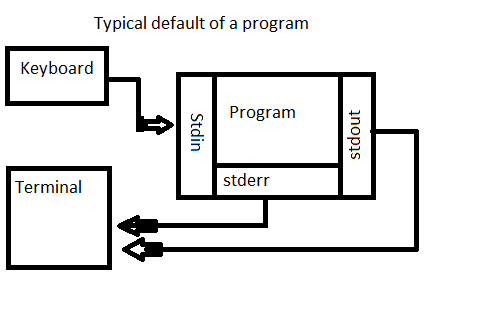
\includegraphics[width=90mm]{stdin_err_out_example.png}
        	\caption{Default configuration.}
        \end{figure}        
     
    \subsection{Redirection}
        File redirection is telling the shell to set stdin, stdout, or stderr to something other than the defaults (i.e. some other file). This is achieved by using the `$>$' and `$<$' characters as part of your command. For example, a common use would be to redirect a program's output to a file when the program typically writes to stdout:
        \commandline{java HelloWold.java $>$ output.txt}
        \vspace{0.3cm}
        Here is a table with some more examples:
        \begin{center}
            \begin{tabular}{|l|l|}
                 \hline
                 program $<$ file1 & stdin is set to file1. \\
                 program $>$ file1 & stdout is set to file1. If file1 does not exist it is created. If it does exist it is overwritten. \\
                 program $>>$ file1 & Same as above but appends to the file instead of overwriting. \\
                 program $2>$ file1 & Same as $>$ but for stderr. \\
                 program $2>>$ file1 & Same as $>>$ but for stderr. \\ \hline
            \end{tabular}
        \end{center}
        
        \vspace{0.5cm}

    \begin{ex} Let's redirect stdout to another file.
        \begin{enumerate}
            \item Navigate to demo/java\_programs/large\_output
            \item Compile and run this program once without redirection.
            \item Now redirect stdout to a file called `output'. NOTE: Using the redirection character will create and open this file for you!
        \end{enumerate}
    \end{ex}

\section{grep}
\textbf{grep} is used to find occurrences of anything that matches a given regular expression in a file. A regular expression, put simply, is a sequence of characters that define a search pattern. Wildcard expansion, for example, uses a regular expression to match file names.

The general form of \textbf{grep} is:
    \commandline{grep options regularExpression file1 file2 ...}
    \vspace{0.15cm}
        The most common options are:
    \begin{center}
    \begin{tabular}{|c|c|}
        \hline
        -r & recursive \\
        -i & case insensitive \\
        -n & line numbers \\ 
        \hline
    \end{tabular}
    \end{center}
    \vspace{0.15cm}
    
    \textbf{grep} is a very useful tool and has a variety of applications in the UNIX environment. Let's give it a try:
    
    \vspace{0.3cm}
    \begin{ex} Find the word `hello' in the output of LargeOutput.java
        \begin{enumerate}
            \item Compile and run LargeOutput.java and redirect it's output to a file called `output'.
            \item Use grep to search for the pattern `hello'. Try writing the search expression in a variety of ways to obtain the same result.
            \item Use the command options to find out the line numbers that `hello' is printed on.
        \end{enumerate}
    \end{ex}
    
\section{Pipes}
Pipes are similar to redirection except that we are changing stdout of one program to now be stdin of another. We can string together as many programs as we would like. Here is the general form:
\commandline{prog1 $|$ prog2 $|$ prog3 ... $|$ progN}
\vspace{0.15cm}

    \begin{figure}[H]
    	\centering
    	\label{tab:directory_tree}
    	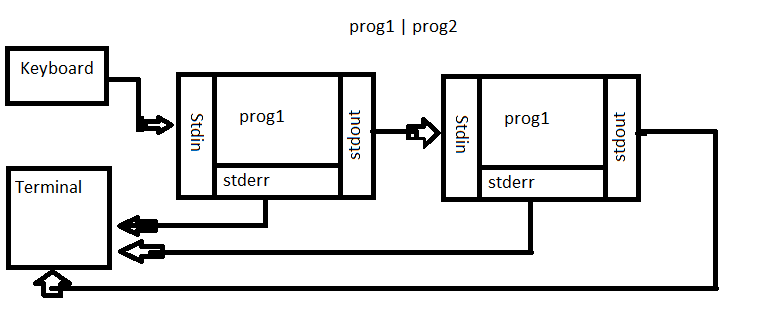
\includegraphics[width=90mm]{pipe_example.png}
    	\caption{The output of prog1 is being piped to the stdin of prog2.}
    \end{figure}

Pipes also have a wide variety of applications in the UNIX environment, but let's take a look at some concrete examples.

Suppose I wanted to view the file listings of a directory, but the directory happens to contain a lot of files. We could pipe the output of \textbf{ls} to another handy program \textbf{less}, and we could view the files in a more reasonable fashion without flooding our console with output.
\commandline{ls -al $\sim$ \textbar \ less}
\vspace{0.15}
This is very helpful when using shells with no scrolling feature.

An extremely powerful command to use with pipes is one we just learn about, \textbf{grep}. We pipe the output of our programs into grep and search for patterns. Say I had written a command awhile back that was rather long (e.g. using \textbf{ssh}\footnote{We will be doing another workshop on this tool and other related tools, but if you're eager to try it out see \textbf{man 1 ssh}.} to log into another machine remotely). To avoid having to type it in again, and potentially make mistakes in the process, we can use bash's builtin command\footnote{Builtin commands are executed directly in the shell itself, instead of an external executable program.} \textbf{history}. By default this command will output entries in our shell's history file, which contains several commands we had previously entered.
\commandline{history \textbar \ grep [search expression]}
\vspace{0.15}

\section{Unlock the true power of your shell: Configuring your .bashrc file.}
\textbf{.bashrc} is a ordinary file with extraordinary capabilities. It's a shell script that Bash runs whenever it is started interactively\footnote{Difference between interactive and non-interactive sessions \url{https://unix.stackexchange.com/questions/50665/what-is-the-difference-between-interactive-shells-login-shells-non-login-shell}}. This allows us to run a bunch of useful commands right when the shell boots up. A useful builtin command commonly found in .bashrc files is \textbf{alias}. 
\commandline{alias [OPTIONS] \ [name[=value]...]}

This command allows a string to be substituted for a word when it is used as the first word of a simple command. If we use this command in our .bashrc file we can ensure that these shortcuts exist whenever we open a new shell! 

You can print out all of your aliases using the \textbf{-p} option. You can also unset aliases using the \textbf{unalias} command. 

\subsection{Creating a .bashrc file}
Navigate to your home directory and create a new file \textbf{.bashrc}. Now open up a text editor and start writing out the commands you want to run when the shell boots up.

We will take a look at an example .bashrc file to get you started, but look online for more example and useful commands to include in your file.

\newpage

\section{Retrospective and Closing Comments}
    If you understand all the content that we just covered then you can now do all of your programming and file managing from the command line. Try to use the command line on your next few projects to master these skills. We have barely scratched the surface, however, and we encourage you to use the \textbf{man} pages and your favorite search engine to look into the tools and topics that we just outlined. Also note that you will learn a lot from friends, teachers, and colleagues in the years to come if you continue in the CSCI program. Good luck out there!
    \\
    \\

\newpage
\begin{thebibliography}{10}
	\bibitem{Figure 1.1} Figure 1.1 found at \url{http://homepage.cs.uri.edu/faculty/hamel/courses/2016/fall2016/csc301/bootcamp/sessions/session-1a.html}
	\bibitem{Figure 1.2} Figure 2 found at \url{http://www.linuxtrainingacademy.com/wp-content/uploads/2014/03/linux-directory-tree.jpg}
\end{thebibliography}



\end{document}
